\chapter{Synopsis}
\section{Hardware Requirements}


\begin{table}[H]
    \fontsize{10}{12}\selectfont
    \caption{Hardware Requirements}
    \label{c1:hardware_requirements}
    \begin{center}
    \begin{tabular}{|p{7cm}|c|c|c|}
        %\hline
        %\multicolumn{4}{|c|}{Country List} \\
        \hline
        \textbf{Processor }& Intel Haswell CPU or IBM POWER8 CPU \\ \hline
        \textbf{Hard Disk Partitions (System and Data)}    &   5 GigaBytes, 15 GigaBytes       \\\hline
        \textbf{Drive}    &   Digital Versatile Disk- Read Only Memory         \\\hline
        \textbf{Screen Display}    &   800 x 600 with 16-bit colors or higher  \\\hline
        \textbf{Random Access Memory}    &   128G \\\hline

    \end{tabular}
    \end{center}
    \end{table}
    
\section{Software Requirements}
Software requirements that are necessary include-
\begin{itemize}
    \item Operating System - Windows 7/greater or MacOS 10.12/greater.
    \item DB : SAP HANA S/4
    \item Programming Languages : SAP ABAP
    \item Application Programming Interfaces : SAP NetWeaver Gateway Client and Open data protocol services.
    \item ABAP Benchmarking Tool : SAP Benchmarking Tool
    \item SAP HANA Cloud : SAP HANA Cloud
    \item SAC : SAP Analytics Cloud
    
\end{itemize}


\section[Methodology]{\textbf{Methodology}}
% Discuss about the methodology you identified to execute the objectives of your project in brief. Methodology is a system of practices, techniques, procedures, and rules used to execute a particular project. You can elaborate the methodology in a later chapter. Here you can present in the form of a flow diagram and explain the methodology in a paragraph.
The steps adopted during the implementation of the Budget Planning Application can
be shown as a three stage pipeline as discussed below :

\begin{itemize}
\item Use of SAP UI5 and SAP Fiori for the deployment of the front-end system. A glimpse
 of the Fiori LaunchPad is shown in the diagram below. It shows the catalogue
 containing a suite of applications customized according to user preferences and
 packages.
 
\begin{figure}[H]
    \centering
        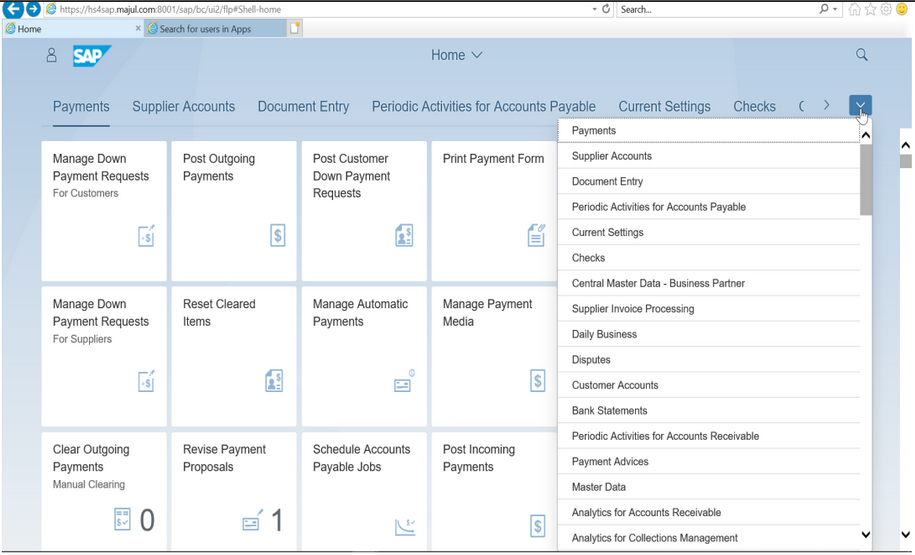
\includegraphics[scale=0.5]{Chapter1/Figures/fiori1.png}	
        \caption{Fiori LaunchPad} 
        \label{fig:fiorilaunchpad}
\end{figure}
    
\item Setting up SAP S/4 HANA databases for collecting and capturing info received
    through the programs. The database can analyze significant volume actual statistics
    in a brief period.
\item Server-side code on the backend built upon SAP ABAP.
\item  To get an expedient solution for data representation, Core Data Services Views are
    supported by the current relational databases and views.
\item  SAP NetWeaver Gateway Client and Open data Protocol are used toh link
    backend with frontend resources.
\end{itemize}

    % \begin{figure}[H]
    %     \centering
    %         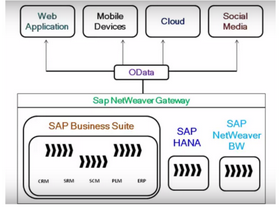
\includegraphics[scale=0.5]{Chapter1/Figures/odata.png}	
    %         \caption{SAP Odata Protocol} 
    %         \label{fig:odataprotocol}
    % \end{figure}
        
%     The figure above shows a high level framework of the different tiers and the connection
%     amongst all components. The Odata and Netweaver Gateway are mainly used for the
%     interlinking of front-end and backend services.


%     The features to be provided include-

%     \begin{itemize}
%         \item Budget requests, reviews and adoption- Manage budgets in a single application

%         \item Operating, capital and grants budgeting - A single application for all budget types

%         \item User configuration - Tailor budget forms, process controls, reports and analytics to your unique budgeting requirements and adapt them to changing requirements
%         \item Personnel cost forecasting - Examine and plan personnel expenditures at a highly granular level to support budgeting, spending plans and collective bargaining
%         \item Modeling and analytics - Powerful modeling tools combined with the strength of SAP Business Objects for reporting, dashboards and ad hoc analysis

% \end{itemize}






% https://www.researchgate.net/profile/Firas-Alomari-3/publication/341642982_An_Overview_of_SAP_Core_Data_Services/links/5eccf21a299bf1c09adf7a33/An-Overview-of-SAP-Core-Data-Services.pdf?origin=publication_detail